\documentclass[a4paper]{jsarticle}

%======================================================================
%		論文のタイトル,著者,日付
%======================================================================

\title{\Huge マルチメディア信号解析\\\huge レポート2\vspace{120mm}}
\author{\Large 濱崎 直紀\vspace{30mm}}
\date{令和元年7月24日}

%======================================================================
%		マクロの読み込みとコマンドの定義
%======================================================================

\usepackage{graphicx}       % eps fileを張り付けるのに必要
%\usepackage[dvipdfmx]{graphicx}     % png等の画像を貼りつけるのに必要
\usepackage{amsmath}
\usepackage{color}
\usepackage{bm}     % 太字を書くのに必要
\usepackage{here}       % その場所に画像を入れるのに必要
\usepackage{comment}        % コメントを挟むのに必要
\usepackage{listings}      % ソースコードを表示するのに必要
\usepackage{jlisting}       % ソースコード内に日本語のコメントアウトがある場合必要(TEX Liveの場合,別途ダウンロードが必要)

%======================================================================
%		本文
%======================================================================

\begin{document}

\begin{titlepage}
\maketitle
\thispagestyle{empty}
\end{titlepage}

\section*{SVM(Support Vector Machine)}
SVM(Support Vector Machine)は機械学習の一つである.
決定境界に最も近いデータであるサポートベクトルと決定境界との距離(マージン)が最大となるように識別境界を決める手法である.
SVMは線形,非線形の両者が存在するが,今回実装したものは線形であるので,以下SVMは線形SVMのことを指すものとする.

\subsection*{概要}
基本的にSVMは2クラス識別であるので,ここでは2クラス識別問題を例に挙げる.\par
各クラスA,Bの存在する境界である超平面をそれぞれ$\bm{w}^T\bm{x}_A+b=1$,$\bm{w}^T\bm{x}_B+b=-1$とおくと,マージン$d$は
\begin{eqnarray}
    d&=&\frac{|\bm{w}^T\bm{x}_{A{\rm or}B}+b|}{\sqrt{||\bm{w}^2||}}\\
    &=&\frac{1}{||\bm{w}||}
\end{eqnarray}
となる.
これを最大化することは,$||\bm{w}||$を最小化することと等価である.\par
また,すべてのデータは境界の超平面の片側に存在することから
\begin{equation}
    y_i(\bm{w}^T\bm{x}+b_i) \geq 1
\end{equation}
\[
    y_i=\begin{cases}
        1 & (x_i \in A)\\
        -1 & (x_i \in B)
    \end{cases}
\]
という制約条件が得られる.\par
よってSVMの目標は「制約条件$y_i(\bm{w}^T\bm{x}+b_i) \geq 1$のもとで$||\bm{w}||$を最小化する」ことである.
しかし,実際には計算の都合上$\frac{1}{2}||\bm{w}||^2$を最小化する問題へと変換する.
\begin{figure}[H]
    \begin{center}
        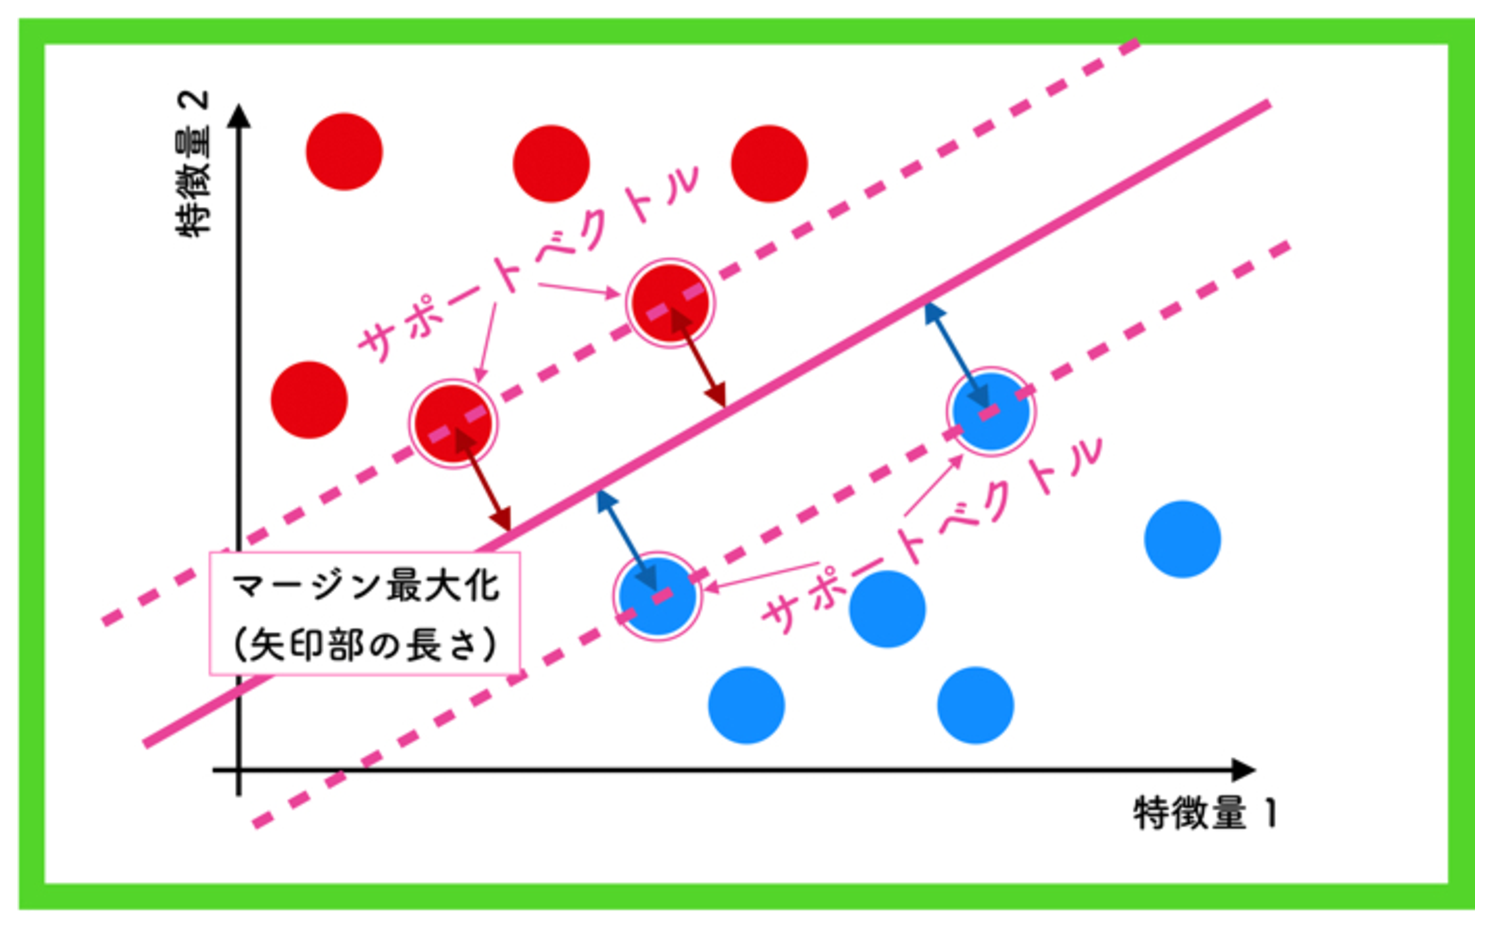
\includegraphics[width=100mm]{./figures/svm/svm.eps}
        \caption{SVMのイメージ図}
    \end{center}
\end{figure}

\subsection*{補足}
SVMはデータの誤分類を許容しない「ハードマージンSVM」と許容する「ソフトマージンSVM」の2種類が存在する.
ハードマージンSVMは,マージン内にデータが存在しないことを前提に考えられており,データがクラス間で重複している場合,識別境界を正確に求められないという問題が生じる可能性がある.
それに対してソフトマージンSVMは,マージン内にデータが存在することやデータの誤分類をある程度許容する代わりに,そのデータにはペナルティを与えるという風に条件を少し緩めることで,多少の重複が存在しても識別できる可能性を上げることを可能としている.\par
では,実際にソフトマージンSVMにおいて,どのようにしてペナルティを与えるのかということに関して簡単に述べる.
まずスラック変数$\zeta$をデータごとに導入する.
$\zeta$はデータが正しく分類されてかつマージン内に存在しない場合は0,正しく分類されているがマージン内に存在する場合は$0<\zeta \leq 1$,誤って分類された場合は$\zeta>1$となる.
そして,マージンの最大化に際して,このスラック変数$\zeta$をペナルティとして与える.
式は以下のようになる.
\begin{equation}
    \zeta_i=|y_i-(\bm{w}^T\bm{x}+b)|
    \label{zeta}
\end{equation}
\begin{equation}
    C\sum_{i=1}^{N}\zeta_i+\frac{1}{2}||\bm{w}||^2 \qquad (C>0)
    \label{margin}
\end{equation}
この式(\ref{margin})を最小化することが目標である.
ここで$C$はペナルティの影響力を制御するパラメータであり,適当に設定する必要がある.
% 式(\ref{zeta})を見て分かる通り,$\zeta$の定義にも$\bm{w}$が含まれている.
誤分類が多くなると式(\ref{margin})の第1項が大きくなるので,最小化しようとするとなるべく誤分類が少なくなるようにパラメータ$\bm{w}$を調整する.
ちなみに,$C \to \infty$とすると,ペナルティの影響力が$\infty$になる,つまり誤分類が全く許容されなくなるので,ハードマージンSVMとなる.\par
ただし,ソフトマージンSVMは与えるペナルティの大きさなどの調整を行う必要があり,少し複雑になることから,今回はハードマージンSVMの実装を行った.

\subsection*{アルゴリズム}
実際に「制約条件$y_i(\bm{w}^T\bm{x}+b_i) \geq 1$のもとで$\frac{1}{2}||\bm{w}||^2$を最小化する」という問題を解いていく.
この問題は多変数関数の最適化問題なので,ラグランジュ乗数$\alpha_i$を導入することで,ラグランジュの未定乗数法に落とし込むことができる.\par
実際にラグランジュ関数は以下のようになる.
\begin{equation}
    L(\bm{w},b,\alpha)=\frac{1}{2}||\bm{w}||^2-\sum_{i=1}^{N}\alpha_i\{t_i(\bm{w}^T\bm{x}_i+b)-1\}
    \label{Lagrange}
\end{equation}
極値条件より,式(\ref{Lagrange})を$\bm{w}$,$b$でそれぞれ偏微分して0とおくと
\begin{equation}
    \left.\frac{\partial L}{\partial \bm{w}}\right|_{\bm{w}=\hat{\bm{w}}}=\hat{\bm{w}}-\sum_{i=1}^{N}\alpha_it_i\bm{x}_i=0
    \label{con1}
\end{equation}
\begin{equation}
    \frac{\partial L}{\partial b}=\sum_{i=1}^{N}\alpha_it_i=0
    \label{con2}
\end{equation}
また,最適性条件より最適解$\hat{\bm{w}}$に対して以下の条件を満たす必要がある.
\begin{equation}
    \nabla L(\hat{\bm{w}},b,\alpha)=\nabla(\frac{1}{2}||\hat{\bm{w}}||^2)-\sum_{i=1}^{N}\alpha_i\nabla\{t_i(\hat{\bm{w}}^T\bm{x}_i+b)-1\}=0
\end{equation}
この式から以下に示す3つの制約条件が得られる.
\begin{equation}
    t_i(\bm{w}^T\bm{x}_i+b)-1 \geq 0
    \label{KKT1}
\end{equation}
\begin{equation}
    \alpha_i \geq 0
    \label{KKT2}
\end{equation}
\begin{equation}
    \alpha_i\{t_i(\bm{w}^T\bm{x}_i+b)-1\}=0
    \label{KKT3}
\end{equation}
式(\ref{KKT1}),(\ref{KKT2}),(\ref{KKT3})はまとめてKKT条件と呼ばれる.\par
式(\ref{con1})より最適解$\hat{\bm{w}}$は
\begin{equation}
    \hat{\bm{w}}=\sum_{i=1}^{N}\alpha_it_i\bm{x}_i
    \label{con1_a}
\end{equation}
式(\ref{con2}),(\ref{con1_a})を式(\ref{Lagrange})に代入すると
\begin{equation}
    L(\hat{\bm{w}},b,\alpha)=\frac{1}{2}||\hat{\bm{w}}||^2-\hat{\bm{w}}^T\sum_{i=1}^{N}\alpha_it_i\bm{x}_i-b\sum_{i=1}^{N}\alpha_it_i+\sum_{i=1}^{N}\alpha_i
\end{equation}
となり,これを$\alpha$の関数と見ると
\begin{eqnarray}
    \tilde{L}(\alpha)&=&\sum_{i=1}^{N}\alpha_i-\frac{1}{2}||\hat{\bm{w}}||^2\\
    &=&\sum_{i=1}^{N}\alpha_i-\frac{1}{2}\sum_{i=1}^{N}\sum_{j=1}^{N}\alpha_i\alpha_jt_it_j\bm{x}_i^T\bm{x}_j
    \label{dual}
\end{eqnarray}
となる.\par
$\bm{w}$はすでに最適化されており,$b$は$\bm{w}$と$\alpha$から一意に定まるので,あとは$\alpha$を最適化すればよい.
主問題は$\frac{1}{2}||\bm{w}||^2$の最小化より,式(\ref{dual})の最大化を行えばよい.
$\alpha$の制約条件としては式(\ref{con2}),(\ref{KKT2})となる.\par
つまり解くべき問題は「制約条件$\sum_{i=1}^{N}\alpha_it_i=0$,$\alpha_i \geq 0$のもとで$\tilde{L}(\alpha)=\sum_{i=1}^{N}\alpha_i-\frac{1}{2}\sum_{i=1}^{N}\sum_{j=1}^{N}\alpha_i\alpha_jt_it_j\bm{x}_i^T\bm{x}_j$を最大化する」ということになる.
このような問題を双対問題と呼ぶ.
\clearpage
\section{Work1}
\subsection*{問題}
何らかの識別問題または回帰問題を設定し,それを機械学習により解く.
さらに,評価データとして,学習データをそのまま使用,学習データとは異なるデータを使用,の2つの場合の性能を比較する.

\subsection{概要}
MNISTの0~9の数字が描かれた画像に対して,機械学習によって描かれている数字を分類する分類器を作成し,その精度を測った.
機械学習の手法にはSVM(Support Vector Machine)を用いた.
以下ではその結果と考察を述べる.

\subsection{結果}
分類の精度を以下に示す.
\begin{table}[H]
    \begin{center}
        \begin{tabular}{cc}
            \hline
            Data & Accuracy\\
            \hline \hline
            Training data & 99.0\%\\
            Test data & 97.9\%\\
            \hline
        \end{tabular}
    \end{center}
\end{table}

\subsection{考察}
実際に精度を測る際に、学習データをそのまま用いて測ることをオープンテスト(open test),学習に使わずに用意しておいたテスト用のデータを用いて測ることをクローズドテスト(closed test)と言う.
今回の分類に関しても両者で精度を測り,結果として,オープンテストでは99.0\%,クローズドテストでは97.9\%という結果が得られた.
比較してみると,オープンテストの方がクローズドテストよりもわずかに高い精度が達成された.
学習の際には学習用のデータをうまく分類できるように学習するため,学習用のデータに対しては精度が高く,それと比較して,未知のデータであるテスト用のデータに対しては低くなるのは妥当な結果であると言えるだろう.\par
今回のように,データを学習用とテスト用のデータに分けて,それぞれのデータを用いて学習とテストを行うことを交差検証と言う.
これは,学習用のデータを分類することに適合し過ぎるあまり,未知のデータに対する分類がうまくいかない(過学習)といった問題を防ぐことが期待される.

\clearpage
\section{Work2}
\subsection*{問題}
統計的パターン認識において,確率密度関数$p(\bm{x}|C_i)$が多次元正規分布で表される場合において,以下の(a)から(c)について示す.\par
ここで,多次元正規分布は以下の式で表される.
\begin{equation*}
    p(\bm{x}|C_i)=\frac{1}{(2\pi)^{d/2}\left|\bm{\sum}_i\right|^{1/2}}\exp\left\{-\frac{1}{2}(\bm{x}-m_i)^t{{\bm{\sum}}_i}^{-1}(\bm{x}-m_i)\right\}
\end{equation*}
\begin{enumerate}
    \renewcommand{\labelenumi}{(\alph{enumi})}
    \item 識別関数$g_i(\bm{x})$は$\bm{x}$の2次関数となる.
    \item 共分散行列が全クラスで等しい($\sum_i=\sum_0$)と仮定した場合,識別関数$g_i(\bm{x})$は$\bm{x}$の一次関数,つまり線形識別関数となる.
    \item $\sum_0$を単位行列であるとし,事前確率が各クラスで等しい($P(C_i)=\frac{1}{c}$;$c$はクラス数)とすると,識別関数$g_i(x)$はNearest Neighbour法と同じ形になる.
    この時のクラス$C_i$のプロトタイプがどのように求められるか示す。
\end{enumerate}

\subsection*{解答}
\begin{enumerate}
    \renewcommand{\labelenumi}{(\alph{enumi})}
    \item
    \begin{align*}
        g_i(\bm{x})&=\log{P(\bm{x}|C_i)}+\log{P(C_i)}\\
        &=\log{\frac{1}{(2\pi)^{d/2}\left|\bm{\sum}_i\right|^{1/2}}\exp\left\{-\frac{1}{2}(\bm{x}-m_i)^t{{\bm{\sum}}_i}^{-1}(\bm{x}-m_i)\right\}+\log{P(C_i)}}\\
        &=-\frac{1}{2}\left\{(\bm{x}-m_i)^t{{\bm{\sum}}_i}^{-1}(\bm{x}-m_i)\right\}-\frac{d}{2}\log{2\pi}-\frac{1}{2}\log{\left|{\bm{\sum}}_i\right|}+\log{P(C_i)}
    \end{align*}
    よって,識別関数$g_i(\bm{x})$は$\bm{x}$の2次関数となる.
    \item
    クラス$i,j$に関して考えると,共分散行列が全クラスで等しいことから
    \begin{equation*}
        p(C_i|\bm{x})=p(C_j|\bm{x})
    \end{equation*}
    つまり
    \begin{equation*}
        p(\bm{x}|C_i)p(C_i)=p(\bm{x}|C_j)p(C_j)
    \end{equation*}
    両辺の対数をとって
    \begin{equation}
        \log{p(\bm{x}|C_i)}+\log{p(C_i)}=\log{p(\bm{x}|C_j)}+\log{p(C_j)}
        \label{eq1}
    \end{equation}
    ここで$\lambda_i=\frac{1}{(2\pi)^{d/2}\left|\bm{\sum}_i\right|^{1/2}}$とおくと$p(\bm{x}|C_i)=\lambda_i\exp\left\{-\frac{1}{2}(\bm{x}-m_i)^t{{\bm{\sum}}_i}^{-1}(\bm{x}-m_i)\right\}$となるので
    \begin{align*}
        \log{p(\bm{x}|C_i)}&=\log{\lambda_i}-\frac{1}{2}(\bm{x}-m_i)^t{{\bm{\sum}}_i}^{-1}(\bm{x}-m_i)\\
        &=\log{\lambda_i}-\frac{1}{2}\left\{\bm{x}^t{{\bm{\sum}}_0}^{-1}\bm{x}-2m_i^t{\bm{\sum}}^{-1}\bm{x}+m_i^t{\bm{\sum}}^{-1}m_i\right\}
    \end{align*}
    これを式(\ref{eq1})に代入すると
    \begin{align*}
        \log\lambda_0-\frac{1}{2}\bm{x}^t{{\bm{\sum}}_0}^{-1}\bm{x}+m_i^t{{\bm{\sum}}_0}^{-1}\bm{x}-\frac{1}{2}m_i^t{{\bm{\sum}}_0}^{-1}m_i+\log{P(C_i)}\\
        =\log\lambda_0-\frac{1}{2}\bm{x}^t{{\bm{\sum}}_0}^{-1}\bm{x}+m_j^t{{\bm{\sum}}_0}^{-1}\bm{x}-\frac{1}{2}m_j^t{{\bm{\sum}}_0}^{-1}m_j+\log{P(C_j)}
    \end{align*}
    よって
    \begin{align*}
        g(\bm{x})&=log{P(C_i|\bm{x})}-log{P(C_j|\bm{x})}\\
        &=m_i^t{{\bm{\sum}}_0}^{-1}\bm{x}-m_j^t{{\bm{\sum}}_0}^{-1}\bm{x}-\frac{1}{2}m_i^t{{\bm{\sum}}_0}^{-1}m_i+\log{P(C_i)}+\frac{1}{2}m_i^t{{\bm{\sum}}_0}^{-1}m_i-\log{P(C_i)}\\
        &=(m_i-m_j)^t{{\bm{\sum}}_0}^{-1}\bm{x}+\left\{-\frac{1}{2}m_i^t{{\bm{\sum}}_0}^{-1}m_i+\log{P(C_i)}+\frac{1}{2}m_i^t{{\bm{\sum}}_0}^{-1}m_i-\log{P(C_i)}\right\}
    \end{align*}
    よって,識別関数$g_i(\bm{x})$は線形識別関数となる.
    \item
    \begin{align*}
        g_i(\bm{x})&=\log{P(C_i|\bm{x})}\\
        &=\log{P(\bm{x}|C_i)}+\log{P(C_i)}\\
        &=\log{P(\bm{x}|C_i)}-\log{c}
    \end{align*}
    ここで,$\sum_0$が単位行列,事前確率が各クラスで等しいということから
    \begin{align*}
        \log{P(\bm{x}|C_i)}&=\log\lambda_i-\frac{1}{2}(\bm{x}-m_i)^t{\bm{\sum}}_i^{-1}(\bm{x}-m_i)\\
        &=\log{\lambda_0}-\frac{1}{2}||\bm{x}-m_i||^2
    \end{align*}
    よって
    \begin{align*}
        g_i(\bm{x})&=\log{P(\bm{x}|C_i)}-\log{c}\\
        &=\log{\lambda_0}-\frac{1}{2}||\bm{x}-m_i||^2-\log{c}\\
        &=-\frac{1}{2}||\bm{x}-m_i||^2+\log{\frac{\lambda_0}{c}}
    \end{align*}
    ゆえに
    \begin{align*}
        \argmax_i{g_i(\bm{x})}&=\argmax_i\left\{-\frac{1}{2}||\bm{x}-m_i||^2+\log{\frac{\lambda_0}{c}}\right\}\\
        &=\argmax_i\left\{-||\bm{x}-m_i||^2\right\}\\
        &=\argmin_i\left\{||\bm{x}-m_i||^2\right\}
    \end{align*}
\end{enumerate}

\clearpage
section*{感想}
今回の実験ではハードマージンSVMの実装しか行えなかった.
パラメータの調整さえできれば,ソフトマージンSVMの方が有用であるように見えるため,実装できていた場合の結果がどうなっていたのかが気になるところではある.
また,SVMの多クラス分類に関しても,いくつかある手法のうちの1つしか実装できなかったので,他の手法を実装できなかったのは課題点として挙げられると思う.

%======================================================================
%		付録
%======================================================================

\clearpage
\appendix
\pagestyle{empty}
% ソースコードの表示に関する設定
\lstset{
    basicstyle={\ttfamily},
    identifierstyle={\small},
    commentstyle={\smallitshape},
    keywordstyle={\small\bfseries},
    ndkeywordstyle={\small},
    stringstyle={\small\ttfamily},
    frame={tb},
    breaklines=true,
    columns=[l]{fullflexible},
    numbers=left,
    xrightmargin=0zw,
    xleftmargin=3zw,
    numberstyle={\scriptsize},
    stepnumber=1,
    numbersep=1zw,
    lineskip=-0.5ex
}
\section{プログラム1}
\begin{lstlisting}[caption=課題1のデータ作成用プログラム]
    import random


    def gauss(mu_x, sigma_x, mu_y, sigma_y, class_label, size):
        data = []
        label = []

        for i in range(size):
            elem = []
            elem.append(random.gauss(mu_x, sigma_x))
            elem.append(random.gauss(mu_y, sigma_y))
            data.append(elem)
            label.append(class_label)

        return data, label
\end{lstlisting}
\clearpage
\section{プログラム2}
\begin{lstlisting}[caption=課題1におけるSVM学習用プログラム]
    import cvxopt
    import matplotlib.pyplot as plt
    import numpy as np
    import os
    from sklearn.model_selection import train_test_split
    import MakeData
    os.chdir(os.path.dirname(os.path.abspath(__file__)))


    # データを学習できる形に変換
    def data_exchange(data1, data2):
        data = data1 + data2        # データを1つにまとめる
        label = label1 + label2     # ラベルを1つにまとめる
        data = np.array(data)       # データ配列をnumpy型に変換
        label = np.array(label)     # ラベル配列をnumpy型に変換
        train_data, test_data, train_label, test_label = train_test_split(data, label, test_size=0.3)       # トレーニング用とテスト用に分ける

        return train_data, test_data, train_label, test_label


    # SVM
    class SVM:
        def __init__(self, data, label):
            self.data = data
            self.label = label
        

        # 線形カーネル
        def kernel(self, x, y):
            return np.dot(x, y)


        # ラグランジュ乗数を二次計画法で求める
        def Lagrange(self, n):
            K = np.zeros((n, n))
            for i in range(n):
                for j in range(n):
                    K[i, j] = self.label[i] * self.label[j] * np.dot(self.data[i], self.data[j])
            Q = cvxopt.matrix(K)
            p = cvxopt.matrix(-np.ones(n))      # -1がn個の列ベクトル
            G = cvxopt.matrix(np.diag([-1.0]*n))        # 対角成分が-1の(n × n)行列
            h = cvxopt.matrix(np.zeros(n))      # 0がn個の列ベクトル
            A = cvxopt.matrix(self.label, (1,n))     # N個の教師信号が要素の行ベクトル(1 × n)
            b = cvxopt.matrix(0.0)      # 定数0.0
            solution = cvxopt.solvers.qp(Q, p, G, h, A, b)       # 二次計画法でラグランジュ乗数alphaを求める

            alpha = np.array(solution['x']).flatten()

            return alpha


        # サポートベクトルを抽出
        def support_vector(self, alpha):
            S = []
            for i in range(len(alpha)):
                if alpha[i] >= 0.00001:
                    S.append(i)
            
            return S


        # wを計算
        def w_cal(self, S, alpha):
            w = np.zeros(2)
            for n in S:
                w += alpha[n] * self.label[n] * self.data[n]
            
            return w

        
        # bを計算
        def b_cal(self, S, alpha):
            _sum = 0
            for n in S:
                tmp = 0
                for m in S:
                    tmp += alpha[m] * self.label[m] * self.kernel(self.data[n], self.data[m])
                _sum += (self.label[n] - tmp)
            b = _sum / len(S)

            return b


        def main(self):
            alpha = self.Lagrange(len(self.data))        # ラグランジュ乗数
            S = self.support_vector(alpha)       # サポートベクトル
            w = self.w_cal(S, alpha)     # w
            b = self.b_cal(S, alpha)        # b

            return w, b, S


    # ラベルごとにデータを分割
    def data_split(data, label):
        cls1 = []
        cls2 = []
        for i in range(len(data)):
            if label[i] == 1:
                cls1.append(data[i])
            elif label[i] == -1:
                cls2.append(data[i])
        
        return cls1, cls2


    def f(x, w, b):
        return np.dot(w, x) + b


    def f_plot(x1, w, b):
        return -(w[0] / w[1]) * x1 - (b / w[1])


    # 精度を計算
    def accuracy(cls1, cls2, w, b):
        num = len(cls1) + len(cls2)
        c = 0
        for i in cls1:
            if f(i, w, b) >= 0:
                c += 1
        for i in cls2:
            if f(i, w, b) < 0:
                c += 1

        acc = c / num

        return acc


    # 結果を描画
    class Draw:
        def __init__(self, data, cls1, cls2, x_min, x_max, y_min, y_max, w, b, S, acc, check):
            self.data = data
            self.cls1 = cls1
            self.cls2 = cls2
            self.x_min = x_min
            self.x_max = x_max
            self.y_min = y_min
            self.y_max = y_max
            self.w = w
            self.b = b
            self.S = S
            self.acc = acc
            self.check = check


        # 結果を描画
        def main(self):
            # 訓練データを描画
            x1, x2 = np.array(self.cls1).transpose()
            plt.plot(x1, x2, 'rx')    
            x1, x2 = np.array(self.cls2).transpose()
            plt.plot(x1, x2, 'bx')

            # サポートベクトルを描画
            if self.check == 'train':
                for n in self.S:
                    plt.scatter(self.data[n,0], self.data[n,1], s=80, c='c', marker='o')
            
            # 識別境界を描画
            x1 = np.linspace(self.x_min, self.x_max, 1000)
            x2 = [f_plot(x, self.w, self.b) for x in x1]
            plt.plot(x1, x2, 'g-')

            plt.xlim(self.x_min, self.x_max)
            plt.ylim(self.y_min, self.y_max)
            plt.text(-25, -25, 'Accuracy : {}%'.format(round(self.acc*100, 2)))
            plt.show()


    if __name__ == '__main__':
        N1 = 100     # クラス1のデータ数
        N2 = 100     # クラス2のデータ数

        # データを作成
        data1, label1 = MakeData.gauss(5, 2.5, 5, 2.5, 1.0, N1)       # クラス1のデータとラベル
        data2, label2 = MakeData.gauss(-5, 2.5, -5, 2.5, -1.0, N2)        # クラス2のデータとラベル
        train_data, test_data, train_label, test_label = data_exchange(data1, data2)

        # SVM
        svm = SVM(train_data, train_label)
        w, b, S = svm.main()

        # トレーニングデータ、テストデータをラベル別に分割
        cls1_train, cls2_train = data_split(train_data, train_label)
        cls1_test, cls2_test = data_split(test_data, test_label)

        # トレーニングデータ、テストデータのそれぞれに対して精度を計算
        acc_train = accuracy(cls1_train, cls2_train, w, b)
        acc_test = accuracy(cls1_test, cls2_test, w, b)
        print('Accuracy for training data : {}'.format(acc_train))
        print('Accuracy for test data : {}'.format(acc_test))
        
        x_min = -30      # xの最小値(描画範囲)
        x_max = 30      # xの最大値(描画範囲)
        y_min = -30      # yの最小値(描画範囲)
        y_max = 30      # yの最大値(描画範囲)

        # トレーニングデータとテストデータに対する結果を描画
        draw_train = Draw(train_data, cls1_train, cls2_train, x_min, x_max, y_min, y_max, w, b, S, acc_train, check='train')
        draw_test = Draw(train_data, cls1_test, cls2_test, x_min, x_max, y_min, y_max, w, b, S, acc_test, check='test')
        draw_train.main()
        draw_test.main()
\end{lstlisting}
\clearpage
\section{プログラム3}
\begin{lstlisting}[caption=課題2のMNISTの数字画像識別におけるSVM学習用プログラム]
    import cv2
    import cvxopt
    import numpy as np
    import os
    import pandas as pd
    import time
    from sklearn.model_selection import train_test_split
    os.chdir(os.path.dirname(os.path.abspath(__file__)))


    # データセットの作成
    class DATASET:
        def __init__(self, num1, num2, num3):
            self.cls = num1
            self.num1 = num2
            self.num2 = num3


        def one_vs_the_rest(self):
            data = []
            label = []
            print('Loading data (positive:{})...'.format(self.cls), end='')
            for num in range(0, 10):
                for root, dirs, files in os.walk('train_img/{}'.format(num)):
                    for f in files:
                        '''
                        # リサイズによる次元削減
                        img = cv2.imread('{}/{}'.format(root, f), 0)
                        dst = cv2.resize(img, dsize=None, fx=0.5, fy=0.5)
                        dst = dst.reshape(-1)
                        data.append(dst)
                        '''
                        data.append(cv2.imread('{}/{}'.format(root, f), 0).reshape(-1))     # 1次元配列に変換してdataに貯めていく
                        if num == self.cls:
                            label.append(1.0)
                        else:
                            label.append(-1.0)
            print('Finish!')
            
            data = np.array(data)
            label = np.array(label)

            data = data / 255.0

            train_data, test_data, train_label, test_label = train_test_split(data, label, test_size=0.9)
            
            return train_data, test_data, train_label, test_label


        def one_vs_one(self):
            data = []
            label = []
            print('Loading data (\"pos\"_\"neg\":{}_{})...'.format(self.num1, self.num2), end='')
            for root, dirs, files in os.walk('train_img/{}'.format(self.num1)):
                for f in files:
                    '''
                    # リサイズによる次元削減
                    img = cv2.imread('{}/{}'.format(root, f), 0)
                    dst = cv2.resize(img, dsize=None, fx=0.5, fy=0.5)
                    dst = dst.reshape(-1)
                    data.append(dst)
                    '''
                    data.append(cv2.imread('{}/{}'.format(root, f), 0).reshape(-1))     # 1次元配列に変換してdataに貯めていく
                    label.append(1.0)
            for root, dirs, files in os.walk('train_img/{}'.format(self.num2)):
                for f in files:
                    '''
                    # リサイズによる次元削減
                    img = cv2.imread('{}/{}'.format(root, f), 0)
                    dst = cv2.resize(img, dsize=None, fx=0.5, fy=0.5)
                    dst = dst.reshape(-1)
                    data.append(dst)
                    '''
                    data.append(cv2.imread('{}/{}'.format(root, f), 0).reshape(-1))     # 1次元配列に変換してdataに貯めていく
                    label.append(-1.0)
            print('Finish!')
            
            data = np.array(data)
            label = np.array(label)

            data = data / 255.0

            train_data, test_data, train_label, test_label = train_test_split(data, label, test_size=0.8)
            
            return train_data, test_data, train_label, test_label


    # SVM
    class SVM:
        def __init__(self, data, label):
            self.data = data
            self.label = label
        

        # 線形カーネル
        def kernel(self, x, y):
            return np.dot(x, y)


        # ラグランジュ乗数を二次計画法で求める
        def Lagrange(self, n):
            K = np.zeros((n, n))
            for i in range(n):
                for j in range(n):
                    K[i, j] = self.label[i] * self.label[j] * np.dot(self.data[i], self.data[j])
            Q = cvxopt.matrix(K)
            p = cvxopt.matrix(-np.ones(n))      # -1がn個の列ベクトル
            G = cvxopt.matrix(np.diag([-1.0]*n))        # 対角成分が-1の(n × n)行列
            h = cvxopt.matrix(np.zeros(n))      # 0がn個の列ベクトル
            A = cvxopt.matrix(self.label, (1,n))     # N個の教師信号が要素の行ベクトル(1 × n)
            b = cvxopt.matrix(0.0)      # 定数0.0
            solution = cvxopt.solvers.qp(Q, p, G, h, A, b)       # 二次計画法でラグランジュ乗数alphaを求める

            alpha = np.array(solution['x']).flatten()

            return alpha


        # サポートベクトルを抽出
        def support_vector(self, alpha):
            S = []
            for i in range(len(alpha)):
                if alpha[i] >= 0.00001:
                    S.append(i)
            
            return S


        # wを計算
        def w_cal(self, S, alpha):
            w = np.zeros(784)
            for n in S:
                w += alpha[n] * self.label[n] * self.data[n]
            
            return w

        
        # bを計算
        def b_cal(self, S, alpha):
            _sum = 0
            for n in S:
                tmp = 0
                for m in S:
                    tmp += alpha[m] * self.label[m] * self.kernel(self.data[n], self.data[m])
                _sum += (self.label[n] - tmp)
            b = _sum / len(S)

            return b


        def main(self):
            alpha = self.Lagrange(len(self.data))        # ラグランジュ乗数
            S = self.support_vector(alpha)       # サポートベクトル
            w = self.w_cal(S, alpha)     # w
            b = self.b_cal(S, alpha)        # b

            return w, b, S


    # ラベルごとにデータを分割
    def data_split(data, label):
        cls1 = []
        cls2 = []
        for i in range(len(data)):
            if label[i] == 1:
                cls1.append(data[i])
            elif label[i] == -1:
                cls2.append(data[i])
        
        return cls1, cls2


    def f(x, w, b):
        return np.dot(w, x) + b


    # 精度を計算
    def accuracy(cls1, cls2, w, b):
        num = len(cls1) + len(cls2)
        c1 = 0
        c2 = 0
        for i in cls1:
            if f(i, w, b) >= 0:
                c1 += 1
            elif f(i, w, b) < 0:
                c2 += 1
        for i in cls2:
            if f(i, w, b) < 0:
                c1 += 1
            elif f(i, w, b) >= 0:
                c2 += 1
        if c1 > c2:
            acc = c1 / num
        elif c1 < c2:
            acc = c2 / num

        return acc


    # 保存
    class SAVE:
        def __init__(self, output_w, output_b, output_acc_train, output_acc_test, processing_time):
            self.output_w = output_w
            self.output_b = output_b
            self.output_acc_train = output_acc_train
            self.output_acc_test = output_acc_test
            self.processing_time = processing_time

        
        def one_vs_the_rest(self):
            # 学習結果のパラメータを保存
            df = pd.DataFrame(self.output_w, index=['0', '1', '2', '3', '4', '5', '6', '7', '8', '9'])
            df['b'] = self.output_b

            dirname = 'classifier'
            if not os.path.exists('{}'.format(dirname)):
                os.mkdir('{}'.format(dirname))

            file_num = 1
            while 1:
                if not os.path.exists('{}/one_versus_the_rest/SVM{}.csv'.format(dirname, file_num)):
                    df.to_csv('{}/one_versus_the_rest/SVM{}.csv'.format(dirname, file_num))
                    print('Save classifier as \"SVM{}.csv\"'.format(file_num))
                    break
                else:
                    file_num += 1

            # 各学習の精度と学習時間を保存
            df = pd.DataFrame({'acc_for_train':self.output_acc_train, 'acc_for_test':self.output_acc_test, 'processing_time':self.processing_time}, index=['0', '1', '2', '3', '4', '5', '6', '7', '8', '9'])
            
            dirname = 'result'
            if not os.path.exists('{}'.format(dirname)):
                os.mkdir('{}'.format(dirname))

            file_num = 1
            while 1:
                if not os.path.exists('{}/one_versus_the_rest/result{}.csv'.format(dirname, file_num)):
                    df.to_csv('{}/one_versus_the_rest/result{}.csv'.format(dirname, file_num))
                    print('Save accuracy and processing time as \"result{}.csv\"'.format(file_num))
                    break
                else:
                    file_num += 1


        def one_vs_one(self):
            # 学習結果のパラメータを保存
            id = []
            for i in range(0, 10):
                for j in range(i+1, 10):
                    id.append('{}_{}'.format(i, j))

            df = pd.DataFrame(self.output_w, index=id)
            df['b'] = self.output_b

            dirname = 'classifier'
            if not os.path.exists('{}'.format(dirname)):
                os.mkdir('{}'.format(dirname))

            file_num = 1
            while 1:
                if not os.path.exists('{}/one_versus_one/SVM{}.csv'.format(dirname, file_num)):
                    df.to_csv('{}/one_versus_one/SVM{}.csv'.format(dirname, file_num))
                    print('Save classifier as \"SVM{}.csv\"'.format(file_num))
                    break
                else:
                    file_num += 1

            # 各学習の精度と学習時間を保存
            df = pd.DataFrame({'acc_for_train':self.output_acc_train, 'acc_for_test':self.output_acc_test, 'processing_time':self.processing_time}, index=id)
            
            dirname = 'result'
            if not os.path.exists('{}'.format(dirname)):
                os.mkdir('{}'.format(dirname))

            file_num = 1
            while 1:
                if not os.path.exists('{}/one_versus_one/result{}.csv'.format(dirname, file_num)):
                    df.to_csv('{}/one_versus_one/result{}.csv'.format(dirname, file_num))
                    print('Save accuracy and processing time as \"result{}.csv\"'.format(file_num))
                    break
                else:
                    file_num += 1


    if __name__ == '__main__':
        while 1:
            svm_type = int(input('\"one_versus_the_rest(0)\" or \"one_versus_one(1)\"? : '))
            if svm_type == 0 or svm_type == 1:
                break
            else:
                print('Error. Please, input \"0\" or \"1\"')
        output_w = []
        output_b = []
        output_acc_train = []
        output_acc_test = []
        processing_time = []

        if svm_type == 0:
            for num in range(0, 10):
                print('==============================')

                dataset_make = DATASET(num, None, None)
                train_data, test_data, train_label, test_label = dataset_make.one_vs_the_rest()

                # SVM
                print('Start learning')
                svm = SVM(train_data, train_label)
                start = time.time()
                w, b, S = svm.main()
                elapsed_time = time.time() - start
                processing_time.append(elapsed_time)
                print('Finish!')

                output_w.append(w)
                output_b.append(b)

                # トレーニングデータ、テストデータをラベル別に分割
                cls1_train, cls2_train = data_split(train_data, train_label)
                cls1_test, cls2_test = data_split(test_data, test_label)

                # トレーニングデータ、テストデータのそれぞれに対して精度を計算
                acc_train = accuracy(cls1_train, cls2_train, w, b)
                output_acc_train.append(acc_train)
                acc_test = accuracy(cls1_test, cls2_test, w, b)
                output_acc_test.append(acc_test)
                print('Accuracy for training data (classify \"{}\") : {}'.format(num, acc_train))
                print('Accuracy for test data (classify \"{}\") : {}'.format(num, acc_test))

            print('==============================')

        elif svm_type == 1:
            for num1 in range(0, 10):
                for num2 in range(num1+1, 10):
                    print('==============================')

                    dataset_make = DATASET(None, num1, num2)
                    train_data, test_data, train_label, test_label = dataset_make.one_vs_one()

                    # SVM
                    print('Start learning')
                    svm = SVM(train_data, train_label)
                    start = time.time()
                    w, b, S = svm.main()
                    elapsed_time = time.time() - start
                    processing_time.append(elapsed_time)
                    print('Finish!')

                    output_w.append(w)
                    output_b.append(b)

                    # トレーニングデータ、テストデータをラベル別に分割
                    cls1_train, cls2_train = data_split(train_data, train_label)
                    cls1_test, cls2_test = data_split(test_data, test_label)

                    # トレーニングデータ、テストデータのそれぞれに対して精度を計算
                    acc_train = accuracy(cls1_train, cls2_train, w, b)
                    output_acc_train.append(acc_train)
                    acc_test = accuracy(cls1_test, cls2_test, w, b)
                    output_acc_test.append(acc_test)
                    print('Accuracy for training data (classify \"{}_{}\") : {}'.format(num1, num2, acc_train))
                    print('Accuracy for test data (classify \"{}_{}\") : {}'.format(num1, num2, acc_test))

            print('==============================')

        # 学習結果のパラメータ、各学習の精度と学習時間を保存
        save = SAVE(output_w, output_b, output_acc_train, output_acc_test, processing_time)
        if svm_type == 0:
            save.one_vs_the_rest()
        elif svm_type == 1:
            save.one_vs_one()
\end{lstlisting}
\clearpage
\section{プログラム4}
\begin{lstlisting}[caption=課題2のMNISTの数字画像識別における識別器の多数決による識別用プログラム]
    import cv2
    import numpy as np
    import os
    import pandas as pd
    from collections import Counter
    os.chdir(os.path.dirname(os.path.abspath(__file__)))


    def dataset():
        data = []
        label = []
        print('Loading data...', end='')
        for num in range(0, 10):
            for root, dirs, files in os.walk('mini_dataset/{}'.format(num)):
                for f in files:
                    data.append(cv2.imread('{}/{}'.format(root, f), 0).reshape(-1))     # 1次元配列に変換してdataに貯めていく
                    label.append(num)
        print('Finish!')

        return data, label


    def f(x, w, b):
        return np.dot(w, x) + b


    def distance(x, w, b):
        return abs(np.dot(w, x) + b) / np.sqrt(np.dot(w, w))


    if __name__ == '__main__':
        while 1:
            svm_type = int(input('\"one_versus_the_rest(0)\" or \"one_versus_one(1)\"? : '))
            if svm_type == 0 or svm_type == 1:
                break
            else:
                print('Error. Please, input \"0\" or \"1\"')

        data, label = dataset()

        if svm_type == 0:
            par = pd.read_csv(filepath_or_buffer="classifier/one_versus_the_rest/SVM0_1.csv", sep=",")
            c = 0
            _sum = 0
            for img in data:
                judge = []
                for num in range(0, 10):
                    w = par.iloc[num, 1:785].values
                    b = par.iloc[num, 785]
                    if f(img, w, b) >= 0:
                        judge.append((num, distance(img, w, b)))
                    elif f(img, w, b) < 0:
                        judge.append((-1, distance(img, w, b)))

                pred = (-1, 1.7976931348623157e+308)
                for i in judge:
                    if i[0] != -1 and i[1] < pred[1]:
                        pred = i

                if pred[0] != -1:
                    if pred[0] == label[_sum]:
                        c += 1
                elif pred[0] == -1:
                    _min = 1.7976931348623157e+308
                    for i in judge:
                        if i[1] < _min:
                            n = i[0]
                            _min = i[1]
                    if n == label[_sum]:
                        c += 1

                _sum += 1

                print('Finish No.{} image'.format(_sum))

        elif svm_type == 1:
            par = pd.read_csv(filepath_or_buffer="classifier/one_versus_one/SVM0_2.csv", sep=",")
            c = 0
            _sum = 0
            c_num = [0]*10
            s_num = [0]*10
            for img in data:
                judge = []
                index = 0
                for i in range(0, 10):
                    for j in range(i+1, 10):
                        w = par.iloc[index, 1:785].values
                        b = par.iloc[index, 785]
                        if f(img, w, b) >= 0:
                            judge.append(i)
                        elif f(img, w, b) < 0:
                            judge.append(j)
                        index += 1

                count = Counter(judge)
                if count.most_common()[0][0] == label[_sum]:
                    c += 1
                    c_num[label[_sum]] += 1

                s_num[label[_sum]] += 1
                _sum += 1

                print('Finish No.{} image'.format(_sum))

        for i in range(0, 10):
            accuracy = c_num[i] / s_num[i]
            print('Accuracy for {} : {}'.format(i, accuracy))
            
        accuracy = c / _sum
        print('Accuracy : {}'.format(accuracy))
\end{lstlisting}

\end{document}